\chapter{Experimental Design and Training Objectives} \label{ch:method}
This chapter defines the formal problem setting, describes the dataset and the data preparation protocol, and specifies the three training objectives of the ablation study. Section~\ref{sec:method:problem} states the mathematical problem formulation. Section~\ref{sec:method:setup} describes the T1DATA dataset and the experimental setup. Section~\ref{sec:method:objectives} details the three training configurations and the research question addressed by each one.

% ================================================================
\section{Problem Formulation} \label{sec:method:problem}
% ================================================================

The forecasting task operates on a univariate continuous glucose monitoring signal sampled at 5-minute intervals. At each time step $t$, a lookback window of $L = 24$ consecutive readings is assembled into an input vector:
\begin{equation}
    \mathbf{x}_t = (g_{t-L+1},\; \ldots,\; g_t) \in \mathbb{R}^{L}
    \label{eq:input}
\end{equation}
where $g_i$ denotes the glucose concentration in mg/dL at step $i$. The window spans 120 minutes of past CGM history.

For the single-step forecasting baseline, the model maps $\mathbf{x}_t$ to a single predicted glucose value at the forecast horizon $H = 12$ steps, corresponding to 60 minutes ahead:
\begin{equation}
    \hat{g}_{t+H} = f_\theta(\mathbf{x}_t)
    \label{eq:singlestep}
\end{equation}

Objective~1 retains the single-step output structure of Equation~\ref{eq:singlestep} but replaces the MSE training criterion with an offset-aware loss function. The input and output structure are unchanged; only the loss used during training differs. The formal definitions of the two evaluated loss functions are given in Section~\ref{sec:bg:losses}.

For multi-step supervision (Objective~2), the output head is extended to predict the complete future trajectory over all $H$ steps simultaneously:
\begin{equation}
    \hat{\mathbf{y}}_t = (\hat{g}_{t+1},\; \ldots,\; \hat{g}_{t+H}) \in \mathbb{R}^{H}
    \label{eq:multistep}
\end{equation}

Forecast-derived event detectors are obtained by applying a threshold criterion to the predicted trajectory $\hat{\mathbf{y}}_t$ within a tolerance window $\tau$, as described in Section~\ref{sec:bg:metrics}. The tolerance sweep in Objective~3 evaluates how detection performance changes as $\tau$ is varied.

For direct binary event classification (Objective~3), a window is labelled positive if the glucose level falls below the hypoglycaemia threshold at any point within the 60-minute prediction horizon:
\begin{equation}
    y_t = \begin{cases} 1 & \text{if } \min_{h=1}^{H}\, g_{t+h} < 70\;\text{mg/dL} \\ 0 & \text{otherwise} \end{cases}
    \label{eq:eventlabel}
\end{equation}

% ================================================================
\section{Dataset and Experimental Setup} \label{sec:method:setup}
% ================================================================

\subsection{The T1DATA Cohort} \label{sec:method:setup:cgm}

The experiments are conducted on the T1DATA dataset~\citep{garciatirado2023t1d}, a randomised crossover clinical trial in which adults with Type~1 diabetes used Dexcom G6 continuous glucose monitoring devices. The dataset provides glucose measurements from 36 anonymised patients recorded at 5-minute intervals over approximately 30 days per patient. Missing values in the raw signal are imputed by linear interpolation before model training.

A defining statistical property of the CGM signal is its high temporal autocorrelation. Across the 36 patients in this cohort, the lag-1 autocorrelation of the raw CGM signal has a mean of 0.985 (SD~0.029), confirming that consecutive 5-minute readings are nearly identical for virtually all patients. This property is the primary driver of the systematic prediction delay described in Chapter~\ref{ch:introduction}: under MSE training, a model that reproduces recent history forward incurs almost no gradient penalty, because the next glucose value is so close to the current one.

For the event detection task, each lookback window is assigned the binary event label of Equation~\ref{eq:eventlabel}: positive if a hypoglycaemic value occurs anywhere within the following 60 minutes, negative otherwise. Because hypoglycaemia is a comparatively rare event, the resulting classification dataset is severely imbalanced, with a cohort-mean positive rate of only 5.7\%. Fig.~\ref{fig:method:class_imbalance} reports both the aggregate class counts and the per-patient breakdown; the positive rate is low throughout the cohort but varies considerably between patients, reflecting differences in individual glycaemic control. An imbalance of this severity is a problem because it would let a model reach high apparent accuracy simply by predicting the negative class almost everywhere, while failing at the actual goal of detecting the rare positive cases. Two design choices counteract this. First, the F2 metric (Section~\ref{sec:bg:metrics:event}) weights recall twice as heavily as precision and therefore rewards the detection of positive events rather than overall accuracy. Second, the direct classifiers are trained with the weighted binary cross-entropy of Section~\ref{sec:bg:losses:bce}, using a positive class weight $w_{+} = N_\text{neg} / N_\text{pos} \approx 16.7$ to offset the imbalance. Both the metric and the loss weighting are derived from the same cohort statistic reported here.

\begin{figure}[tbp]
    \centering
    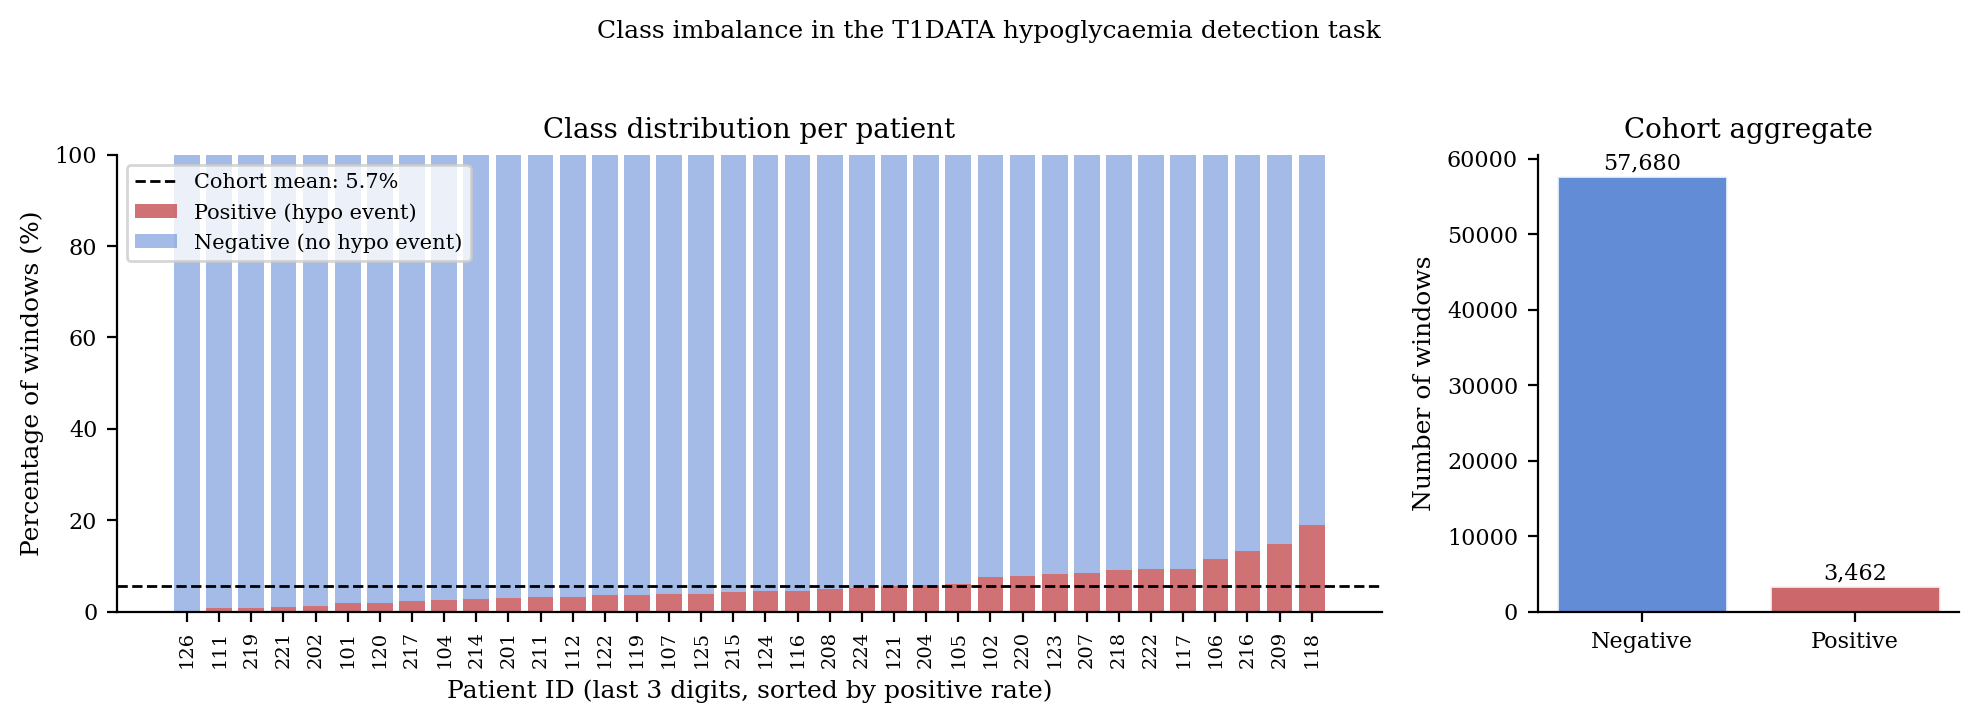
\includegraphics[width=\textwidth]{class_imbalance.png}
    \caption{Class distribution of the hypoglycaemia detection task across the 36-patient T1DATA cohort. \textit{Left:} stacked bars show the percentage of positive (red, glucose falls below 70~mg/dL within the next 60~min) and negative (blue) windows per patient, sorted by ascending positive rate; the dashed line marks the cohort mean of 5.7\%. \textit{Right:} absolute window counts aggregated across all patients (57{,}680 negative vs.\ 3{,}462 positive).}
    \label{fig:method:class_imbalance}
\end{figure}

\subsection{Train/Val/Test Splits and Hyperparameter Optimisation} \label{sec:method:setup:splits}

Each patient's time series is partitioned chronologically into training (60\%), validation (20\%), and test (20\%) sets. Temporal order is strictly preserved to prevent future information from entering the training set. All models are trained and evaluated independently per patient, and the reported metrics are cohort means across all 36 patients.

Hyperparameters are determined using the Optuna automated search framework~\citep{akiba2019optuna} with 50 trials conducted on a single designated tuning patient (ID~85202). Restricting the search to one patient reduces the computational cost by a factor of 36 relative to a full-cohort search; this is a pragmatic compromise, and the resulting configuration may not be globally optimal for all patients (see Section~\ref{sec:conc:limitations}). The resulting configuration is then fixed for all three research objectives; only the loss function or output head changes between objectives, so that any observed performance difference can be attributed to that single change rather than to incidental differences in tuning.

Tab.~\ref{tab:method:hyperparams} reports the resulting configurations. The search converged on markedly different settings for the two architectures: the LSTM uses a comparatively wide hidden state with moderate dropout across few layers, whereas PatchTST uses a smaller model dimension distributed over more layers with almost no dropout, together with the attention-specific parameters (feed-forward dimension and number of heads) that have no LSTM counterpart and are therefore left blank. The input and output dimensions, in contrast, are not tuned but fixed by the problem definition of Section~\ref{sec:method:problem} and shared by both models: a lookback window of 24 steps and a forecast horizon of 12 steps. All models are optimised with the AdamW optimiser~\citep{loshchilov2019adamw}.

\begin{table}[tbp]
\centering
\caption[Optuna-tuned hyperparameters]{Optuna-tuned hyperparameters for the LSTM and PatchTST architectures. The search was conducted on the validation set of patient 85202 only. Identical hyperparameters are used for all training objectives (MSE, Bounded-Lag, Soft-DTW, Multi-Step); only the loss function or output head is modified per objective.}
\label{tab:method:hyperparams}
\begin{tabular}{lrr}
\toprule
Hyperparameter & LSTM & PatchTST \\
\midrule
Hidden size / $d_\text{model}$      & 256     & 64 \\
Number of layers                     & 2       & 3 \\
Dropout                              & 0.159   & 0.025 \\
Learning rate                        & $9.61 \times 10^{-4}$ & $1.21 \times 10^{-4}$ \\
Batch size                           & 128     & 128 \\
Feed-forward dim.\ ($d_\text{ff}$)  & ---     & 256 \\
Attention heads ($h$)                & ---     & 4 \\
Lookback window                      & \multicolumn{2}{c}{24 steps (120 min)} \\
Forecast horizon                     & \multicolumn{2}{c}{12 steps (60 min)} \\
Optuna trials                        & \multicolumn{2}{c}{50} \\
\bottomrule
\end{tabular}
\end{table}


% ================================================================
\section{Training Objectives} \label{sec:method:objectives}
% ================================================================

All three objectives follow a controlled ablation design: exactly one component of the training configuration is modified per objective while all other settings remain fixed. This ensures that observed differences in performance can be attributed to the specific change under investigation. Each objective operationalises one of the three research questions posed in Chapter~\ref{ch:introduction}: its experimental design is specified here, its results are reported in the corresponding section of Chapter~\ref{ch:experiments}, and the question itself is answered in Chapter~\ref{ch:conclusions}.

\subsection{Objective 1: Offset-Aware Loss Functions} \label{sec:method:obj1}

Objective~1 addresses the first research question (Chapter~\ref{ch:introduction}): whether replacing the standard MSE loss with a loss function that tolerates small temporal offsets reduces the systematic prediction delay, and whether any such temporal gain improves hypoglycaemia event detection. Both architectures are retrained twice under otherwise identical conditions: once using the Bounded-Lag loss (Section~\ref{sec:bg:losses:bl}) and once using the Soft-DTW loss (Section~\ref{sec:bg:losses:sdtw}). Concretely, the experiment tests whether an offset-aware training objective produces predictions whose 70~mg/dL threshold crossings fall closer in time to the true hypoglycaemia onset.

\subsection{Objective 2: Multi-Step Supervision} \label{sec:method:obj2}

Objective~2 addresses the second research question (Chapter~\ref{ch:introduction}): whether supervising the model on the complete 60-minute forecast trajectory, rather than a single endpoint, reduces the prediction delay and improves event detection. The output at $t+H$ is replaced by 12 simultaneous predictions at $t+1, \ldots, t+H$, and the MSE loss is computed uniformly across all predicted steps. Because earlier steps in the output sequence carry direct temporal feedback about the near future, the expectation is that this broader supervision signal anchors the predicted trajectory in time and thereby reduces the systematic delay.

\subsection{Objective 3: Event-Centric Evaluation} \label{sec:method:obj3}

Objective~3 addresses the third research question (Chapter~\ref{ch:introduction}): whether task-specific binary classifiers trained directly on the event label outperform threshold-based detection derived from regression forecasts. It approaches event detection from three complementary perspectives, which together establish not only whether the classifiers detect events but why forecast-derived detection falls short and what kind of warning the classifiers provide.

The first sweeps the event detection tolerance window $\tau$ from 0 to 60 minutes in 5-minute steps for all forecast-derived detectors. This quantifies how detection performance changes as the acceptance window is widened, separating the contribution of timing mismatch from other sources of detection failure.

The second trains dedicated binary classifiers end-to-end on the event label $y_t$ of Equation~\ref{eq:eventlabel}. The classifier reuses the same LSTM and PatchTST backbones as the forecasting models (Section~\ref{sec:bg:models}) but replaces the regression head with a single output passed through a sigmoid, so that the model emits a probability $\hat{p}_t \in [0,1]$ that the window beginning at $t$ contains a hypoglycaemic step within the next 60 minutes. Training uses the weighted binary cross-entropy loss of Section~\ref{sec:bg:losses:bce}, with the positive class weight set to $w_{+} \approx 16.7$, the negative-to-positive window ratio of the cohort (Section~\ref{sec:method:setup:cgm}). At evaluation time a window is flagged positive when $\hat{p}_t > 0.5$, and the confusion-matrix counts are accumulated per window against $y_t$; the resulting precision, recall, and $F_\beta$ scores (Section~\ref{sec:bg:metrics:event}) are compared against those of the threshold-based forecast detectors to assess whether a task-specific training objective addresses the detection gap.

The third examines the lead-time distribution of true-positive detections from the direct classifiers. Lead time is defined as the elapsed time from alarm issuance to the first hypoglycaemic step in the prediction window. This analysis quantifies not only whether the classifiers detect events, but at what point relative to event onset — distinguishing alarms issued before the hypoglycaemic episode from those issued at the moment it has already begun.
